\section{Grundlagen der Objektorientierung}

\subsection{Elemente der objektorientierten Programmierung}
\begin{itemize}
    \item Klassen (Objekte)
    \item Vererbung
    \item Kapselung
    \item Polymorphie
\end{itemize}

\subsection{Klassen}
\begin{itemize}
    \item Klassen sind Vorlagen zur Erzeugung von Objekten.
    \item Objekte werden zur Laufzeit eines Programms erzeugt.
    \item Klassen definieren Attribute (Eigenschaften) und Methoden eines Objekts.
    \item Lokale und globale Klassen\footcite[Vgl.][S. 4]{zaidiSAPABAPObjects2019}. 
    \item Beispiel Klasse Auto
    \begin{itemize}
        \item Besitzt Attribute z. B. Farbe oder Kilometerstand
        \item Definiert Methoden wie
        \begin{itemize}
            \item Starten() - Startet den Motor
            \item TankAnzeigen() - Zeigt Füllstand des Motors
        \end{itemize}
    \end{itemize}
\end{itemize}

% Abbildung Klassendiagramm
\begin{figure}
    \includegraphics[width=\linewidth]{bilder/klassendiagramm.png}
    %\includegraphics[width=\linewidth]{klassendiagramm}
    % Müssen wir uns nochmal anschauen, wie wir das am besten machen...
    \caption{Beispiel eines komplexeren Klassendiagramms, Quelle: \footcite[][]{wikipediabenutzerUMLKlassendiagramm}}
    %\caption{Beispiel eines komplexeren Klassendiagramms, Quelle: \textcite{wikipediabenutzerUMLKlassendiagramm}}
    \label{fig:bsp_klassendiagramm}
\end{figure}

\subsection{Vererbung}
\begin{itemize}
    \item Ermöglicht Nutzung verschiedener Eigenschaften eines Objekts
    \item Vererbung von
    \begin{itemize}
        \item Methoden
        \item Variablen
        \item Konstanten
    \end{itemize}
    \item Abhängig von Sichtbarkeit (z. B. Public / Private)
\end{itemize}

\subsection{Kapselung}
\begin{itemize}
    \item Zugriff nur über definierte Methoden (Getters / Setters)
    \item Kontrollierte Ein- und Ausgabe von Werten (z. B. durch Exception)
    \item Innerer Aufbau bleibt verborgen
\end{itemize}

% Hier Tabelle mit Zugriffsrechten
\begin{table}[h!]
    \begin{tabular}{ l l }
        \hline
        \textbf{Zugriffsrecht} & \textbf{Bedeutung} \\ \hline
        Public & Zugriff von überall möglich \\ \hline
        Private & Zugriff nur innerhalb der eigenen Klasse \\ \hline 
        Protected & Zugriff im selben Paket und Subklassen \\ \hline
        Package & Zugriff nur von Klassen im selben Paket (von ABAP \underline{nicht} unterstützt) \\ 
        \hline
    \end{tabular}
    \caption{Tabelle mit Übersicht zu Sichtbarkeiten}
    \label{table:1}
\end{table}

\subsection{Polymorphie}
\begin{itemize}
    \item Liskovsches Substitutionsprinzip
    \item Generalisierter Code in Basisklassen und Verwendung in Subklassen
    \item Abgeleitetes Objekt tritt an die Stelle eines Objekts aus Basisklasse (Up-Cast)
    \item Bezeichner kann anhängig von seiner Verwendung Objekte von div. Datentypen annehmen
\end{itemize}
\newpage
